JavaScript was introduced 1995 with the intention to solve small tasks such as validation of input data and small animations \parencite{Moller2018} and is today well supported in virtually all web browsers on both desktop and mobile \parencite{Zakai2011}. According to \textcite{TiwariSolihin2012} more than 95\% of all web pages are viewed with JavaScript enabled web browsers and more than 99\% of all web sites use JavaScript. While web apps have an advantage of portability compared to native mobile apps, the dynamic typing and prototypes features of JavaScript makes it execution inefficient \parencite{ParkJungMoon2015}.

\subsubsection*{Optimizing/ations/JIT}

The manufacturers of web browsers has in the last few years focused on optimizing JavaScript performance in different ways, such as introducing ''Just-In-Time'' (JIT) compilers \parencite{HerreraChenLavoieHendren2018}.

Previously we had characters/strings being parsed into an abstract syntax tree (AST) that was then used to generate bytecode that was run with an interpreter.

optimizations starts with looking at the execution and generate optimized versions of the course, this is called just in time compliations. some browsers (safari) has up to 4 levels of optimizations. not a good optimized. webassembly needs this.

%https://blog.mozilla.org/luke/2014/01/14/asm-js-aot-compilation-and-startup-performance/

parse, compile + optimize, re-optimize, execute, garbage collection

% https://hacks.mozilla.org/2017/02/what-makes-webassembly-fast/

- the web has become the most ubiquitous application platform ever, and yet by historical accident the only natively supported programming language for that platform

- a new portable size and load-time-efficient format suitable



JavaScript as the assembly of the web. Not very good. Invented in 10 days. Never designed as a compilation target.



''One popular way of accelerating JavaScript is using the just-in-time compilation (JITC), which translates the JavaScript source code to the machine code at runtime. Unfortunately, JavaScript JITC for web apps suffers from the parsing and compilation overhead seriously, which offsets the performance gain of executing the compiled code.'' \parencite{ParkJungMoon2015}


A major problem with optimizing is that fact that JavaScript is a loosely typed language, which means that the interpreter needs to be able to store any type of data in any variable. If the interpreter instead would be able to distinguish between which type of data each variable can store, it would be much easier to optimize. This is asm.js.

\clearpage

\begin{figure}[!h]
\centering
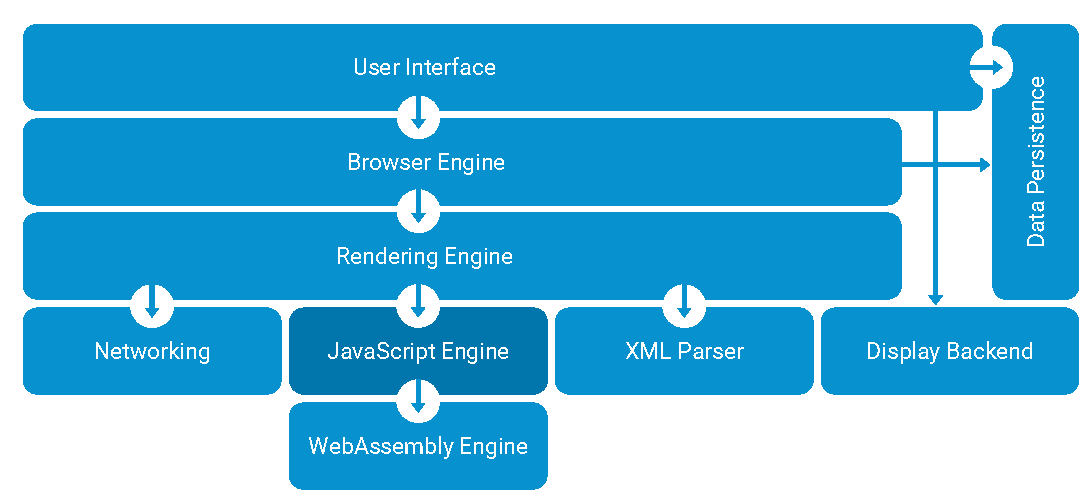
\includegraphics[width=16cm,keepaspectratio]{../Figures/reference-architecture}
\caption{Web browser reference architecture. Adapted from \textcite{GrosskurthGodfrey2005}.}
\label{reference-architecture}
\end{figure}

\begin{figure}[!h]
\centering

\includegraphics[width=16cm,keepaspectratio]{../Figures/javascript-optimization}
\caption{JavaScript execution tiers. Adapted from \textcite{ParkKimMoon2017}.}
\label{javascript-optimization}
\end{figure}

\subsubsection*{AOT}

\subsubsection*{TypeScript}

TypeScript \hl{REF} is a superset of JavaScript that adds type information. Type information allows the programmer to see mistakes sooner during the development phase rather than later in runtime.

\lstinputlisting[label=listing:typescript,language=JavaScript,caption=prime.ts]{../Listings/isprime.ts}

This does not directly solve the problem, but decreases the number of runtime errors, and enables future backend optimizations such as improved guesses by the JIT-compiler.

% if there should be any subsubsection section shown in the table of contents it should be asm.js
\subsubsection{asm.js}

- if the browser understands "use asm" it skips many of the optimization steps. it it doesnt it simply ignores it. asm.js is pretty verbose and thus has some overhead.

- memory in both asm.js and webassembly is a continious array of bytes. the webassembly array is actually shared with javascript so you can read and write to it from both languages

- works as a stack machine in a assembly language

- module interchangeable

- show examles in node? its available since node 8

- working with strings are harder 17m

% https://www.youtube.com/watch?v=pBYqen3B2gc

- a stack machine 4 types, 67 instructions. designed to support streaming compilation, simple validation rules. exports / imports functions. shared linear memory with javascript



Manages its own memory by using a typed buffer instead of relying on garbage collection.

>Much of this performance gain over normal JavaScript is due to 100\% type consistency and virtually no garbage collection (memory is manually managed in a large typed array). This simpler model with no dynamic behavior, no memory allocation or deallocation, just a narrow set of well-defined integer and floating point operations enables much greater performance and potential for optimization.[citation needed] -w

>In the generated code, the variable MEM8 is actually a byte-by-byte "view" of a typed buffer, which serves as the "heap" of the asm.js code. -w





Asm.js is a subset of JavaScript that is focused on performance. It's works 

asm.js is a subset of JavaScript that is known to be heavily optimized. The main part of the optimization is ...

https://en.wikipedia.org/wiki/Asm.js

''A key development here is asm.js,1 which in 2013 was introduced in the Firefox browser. The idea behind asm.js is that JavaScript is slow because it is very dynamic and com- plex, so if we define a subset of JavaScript that is simple, it could be far more easily optimized,'' \parencite{Zakai2018}

\lstinputlisting[label=listing:asmjs,language=JavaScript,caption=asm.js]{../Listings/asm.js}
\listing[abc]{../Listings/isprime.ts}
%\listing[Some listing caption]{asm.js}

%\figure[Some figure caption]{javascript-optimization}

Listing \ref{listing:asmjs} shows an implementation of a C string calculation length function written in asm.js.

There are transpilers between JavaScript and asm.js such as EmScripten.

\textcite{ReiserBlaser2017} describes that there is always a desire for higher performance in web applications.
\textcite{Zakai2018} describes JavaScript as an obstacle for demanding high-performing apps. 
\textcite{HaasRossbergSchuffTitzerHolmanGohmanWagnerZakaiBastien2017} notes that while the web has given rise to demanding web apps JavaScript as a language, being the only programming language available in web browsers, is not very well equipped to support such applications.

%\lstinputlisting[label=prototype,language=JavaScript,caption=prototype.js]{../Listings/prototype.js}
